\documentclass{article}
\usepackage[table]{xcolor}
\usepackage{graphicx}
\usepackage{multicol}

\title{Some work with the Adult data set}


\begin{document}

\section{Introduction}

Put the introduction here. Talk about the assignments in DATASCI400 that led to the creation of this project

\section{The Dataset}

The project uses the Adult dataset from the UCI machine learning archive.  This is where I will put the graphs and descriptive statisitics from the dataset.

\section{The Models}

I created several models for this project.  Some of the models were used in DATASCI400 while others were part of later courses that I have retroactively applied here.

In all cases I used the default probability threshold of 0.5.  This consistency is for making comparisons across models, and is in no way a final decision on the proper threshold, which would be based on some theoretical cost-benefit analysis.

\subsection{Logistic Model with Everything}

The first model is a simple Logistic model using everything in the data set except for education, which is redundant with education number, and fnlwt, the census estimated weights of each observation.  For a naive attempt, this model actually performs okay, with an accuracy of 84\% and a recall of 60\%.  There is certainly room for improvement, so let us see if subsequent models perform better.

	\begin{multicols}{2}
	\begin{center}
	
	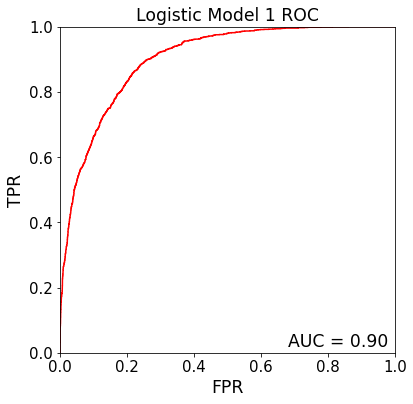
\includegraphics[scale = .4]{Logistic Model 1_ROC}
	
	\columnbreak
	
	\input{Logistic Model 1_CM.txt}
	
	\vspace{0.2 in}
	
	\input{Logistic Model 1_scores.txt}
	
	
	\end{center}
	\end{multicols}

\subsection{Logistic Model With Everything and \\ Synthetically Balanced Classes}

While the class imbalance is not extreme, it is present, so perhaps balancing the classes would lead to improved results.  While it certainly returns different results, whether or not it is superior is in the eye of the beholder.  Recall increases by 23\% and F1 increases 2\% over the unbalanced model, but at the cost a 12\% increase in the false positive rate.  This model may be better than the above model, depending on the benefit of a true positive versus the cost of a false positive.

	\begin{multicols}{2}
	\begin{center}
	
	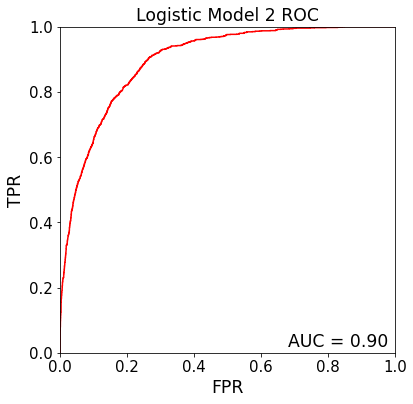
\includegraphics[scale = .4]{Logistic Model 2_ROC}
	
	\columnbreak
	
	\input{Logistic Model 2_CM.txt}
	
	\vspace{0.2 in}
	
	\input{Logistic Model 2_scores.txt}
	
	
	\end{center}
	\end{multicols}



\end{document}